\subsection{Painting Rectification}
We manage to perform a very accurate rectification when the painting retrieval is able to correctly fetch the painting entry from our database. In this case, not only we have the correct correspondence of paintings, but we can also exploit the descriptors obtained from ORB to compute an extremely accurate homography matrix, thanks to the large number of keypoints, to then compute the projective transformation. We see an example in fig.~\ref{fig:rectification_ex}.

\begin{figure}[h!]
    \centering
    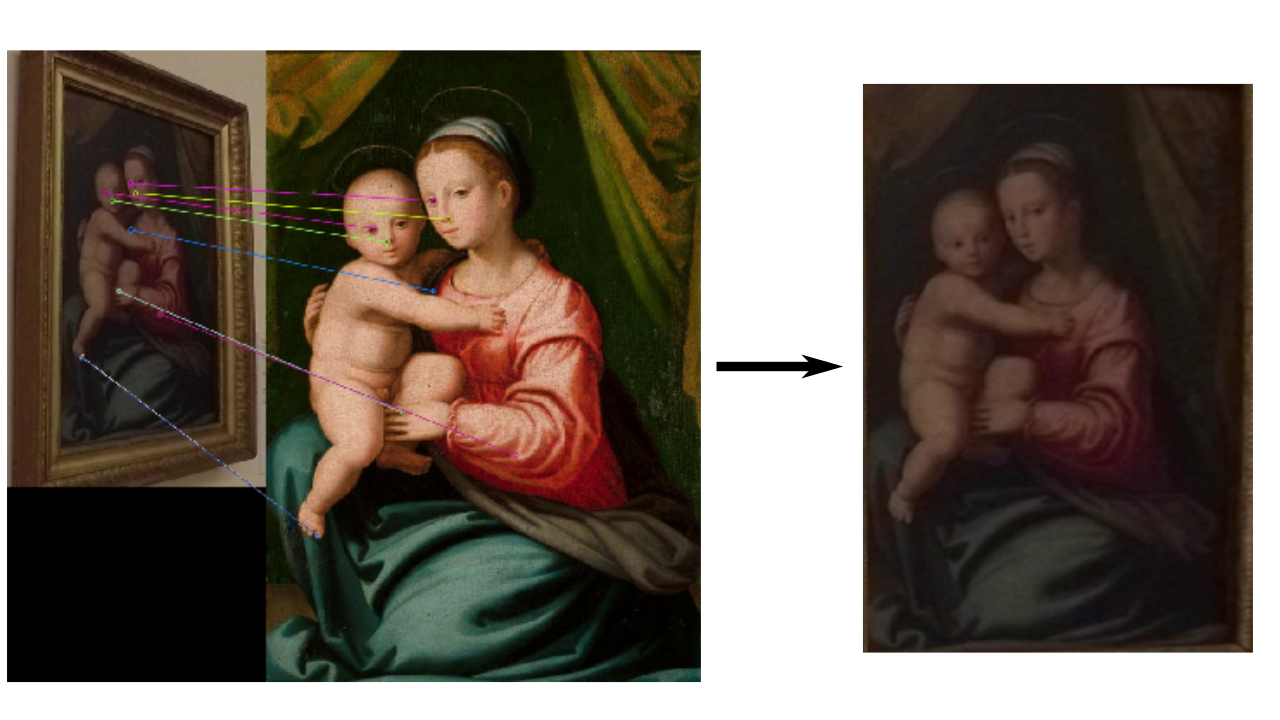
\includegraphics[width=.49\textwidth]{pictures/painting_rectification/rectification.png}
    \caption{example of painting rectification}
    \label{fig:rectification_ex}
\end{figure}

When the retrieval fails, for the lack of descriptors or when the painting is missing from the database, we use Harris Corner Detector~\cite{harris-corner} to find the corners of the painting and use them as source points for our homography matrix. This method has a worse performance than the descriptors method, since the corners are not always precise.
